\section{Frequency mode 01}
\label{sec:fm01}

\subsection{Overview}
\label{sec:fm01:overview}
Frequency mode~01 monitors two bands, $501.180$--$501.580\,\mathrm{GHz}$ and
$501.980$--$502.380\,\mathrm{GHz}$. Its main use is retrievals of \chem{O_3},
\chem{ClO} and \chem{N_2O}. This ozone product has previously been used as
the main \smr\ ozone product despite the weak line and thereby noisy profiles.
Spectra from this observation mode are shown in Figure~\ref{fig:spectra:01}.
We hope that this reprocessing will make the FM~02 ozone the main product.


\begin{figure}[ht]
    \centering
    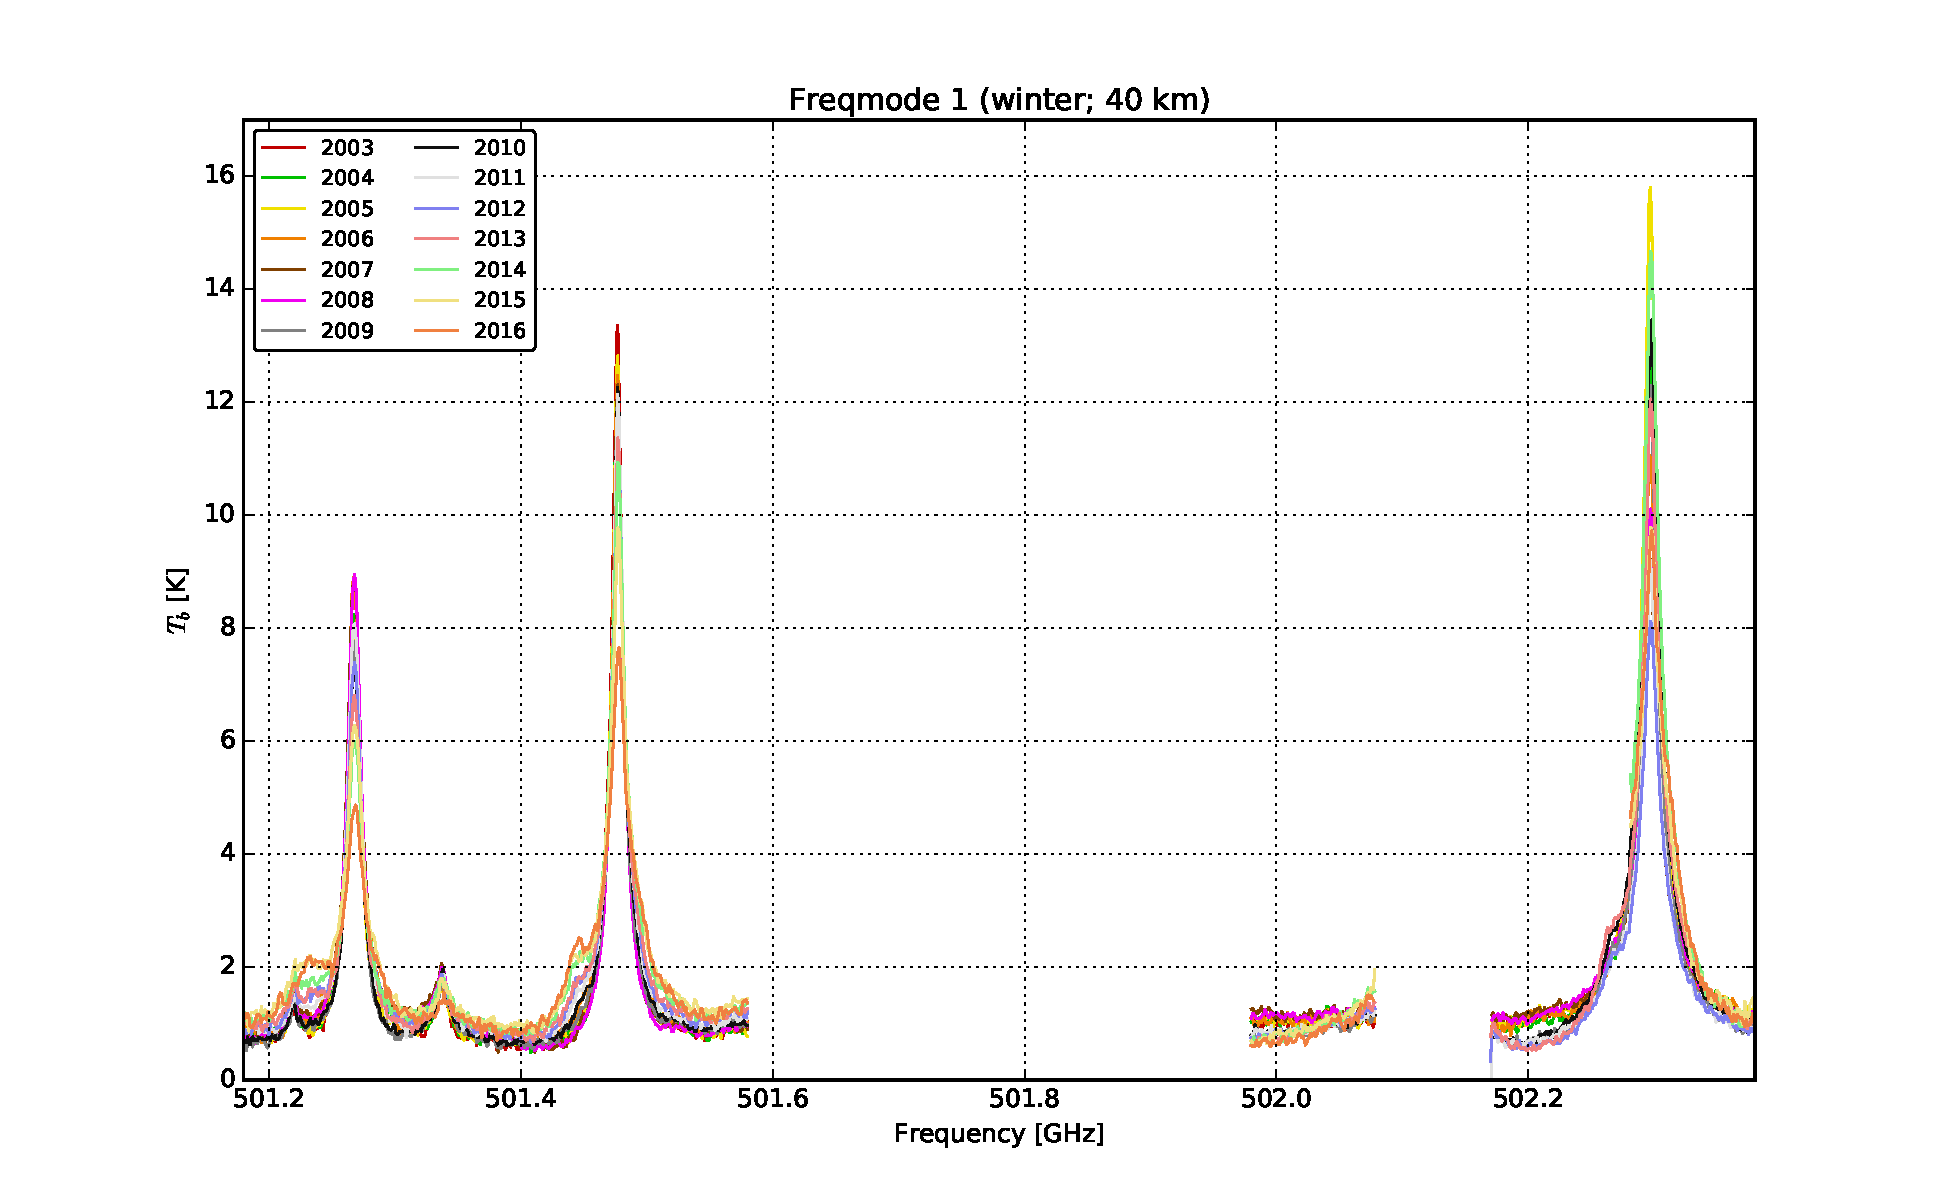
\includegraphics[width=0.95\textwidth]{../DDS/figures/spectra/fm_01_spectra_winter}
    \caption{Annual median spectra for FM~01 for altitude interval 35--45~km at
        equatorial latitudes during the arctic winter.
    }\label{fig:spectra:01}
\end{figure}


\subsection{Comparison of retrieved profiles}
\label{sec:fm01:comparison}


%%%%%%
% O3 %
%%%%%%

\subsubsection{\chem{O_3}}
\label{sec:fm01:comparison:O3}
The retrievals for \chem{O_3} have been compared with data from the MIPAS, MLS,
OSIRIS and SAGE~III instruments. Annual average differences to these
instruments are shown in Figure~\ref{fig:fm01:O3:profiles}. In
Figure~\ref{fig:fm01:O3:scatter} individual retrievals for the instruments for
2003--2019 (depending on the instrument)  are plotted against the
retrievals from the new and old versions of the \smr\ processing chain. The
results show a considerable improvement with the updated version of the
processing, with much better overall correlation and coherency, and most of the
systematic under estimation having been removed compared to all instruments
except for SAGE~III.  Compared to SAGE~III, the results were bad for \smr~v2.X,
but are even worse for \smr~v3. This may be attributed to the fact that the
collocated measurements for SAGE~III are all from altitude range $40$--$50$~km,
which is the upper range of altitudes for this frequency mode, and the lower
range for the SAGE~III instrument, as seen in
Figure~\ref{fig:fm01:O3:profiles:SAGEIII}.

A clear drift in the results is seen after 2009 and data from 2010--2017
should be treated with extreme care. The reason for the drift has now been
identified as an instrument problem where an unstable oscillator has widened
the instrument line-profile. This may be possible to correct for in a later
version of the data but will require an in depth study of the problem and
possible corrections strategies. Data from 2018 and onward seems to be free
of this problem thanks to a retuning of some parameters on-board the
satellite. The useful range for the product and the vertical resolution is
shown in Figure~\ref{fig:fm01:O3:mr_avk}. Based on an analysis of the
averaging kernels and comparisons with the other instruments the product is
useful for the range 19--50~km with a resolution of around 5~km. The
resolution is slightly degraded compared to the version 2.x product due to
increased vertical correlation used to stabilise the retrievals.

\begin{figure}[tbhp]
    \centering
    \begin{subfigure}[b]{0.49\textwidth}
        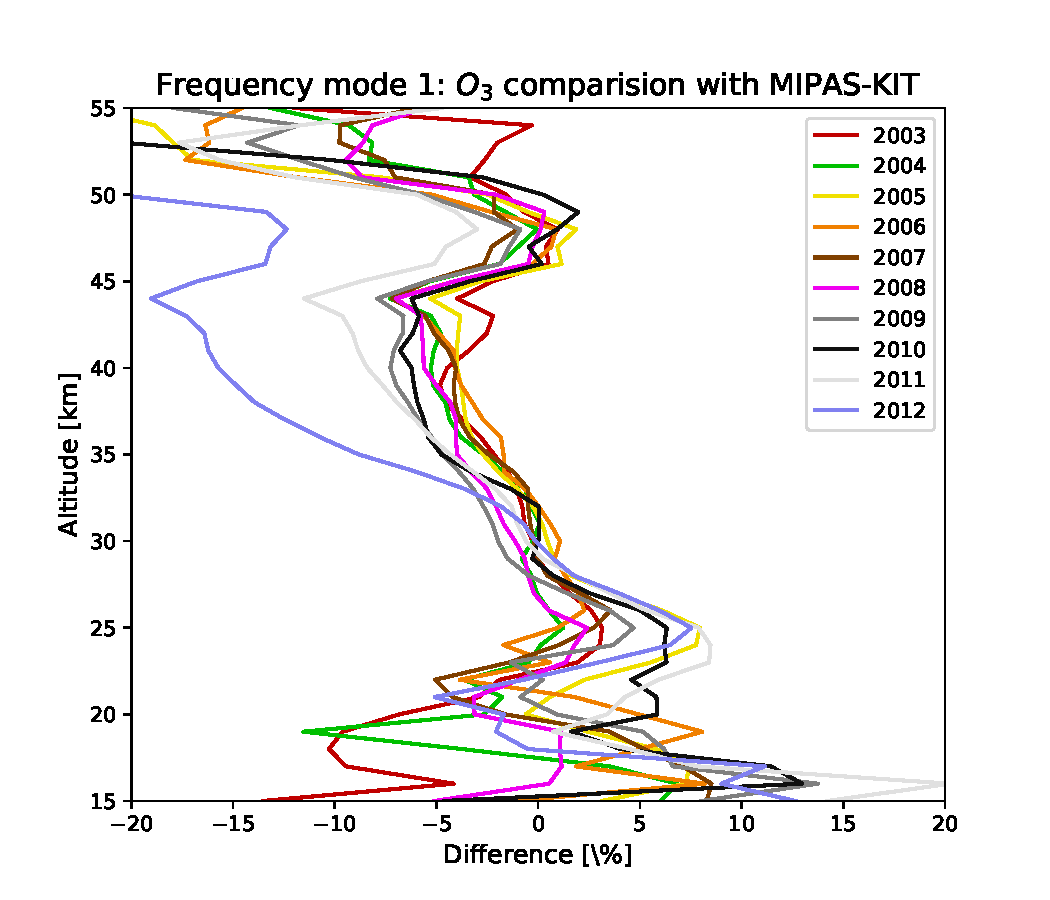
\includegraphics[width=\textwidth]{ALL-Strat-v3_0_0_fm1_O3_perdiff_mipas}
        \caption{average difference to MIPAS}
        \label{fig:fm01:O3:profiles:MIPAS}
    \end{subfigure}
    \,
    \begin{subfigure}[b]{0.49\textwidth}
        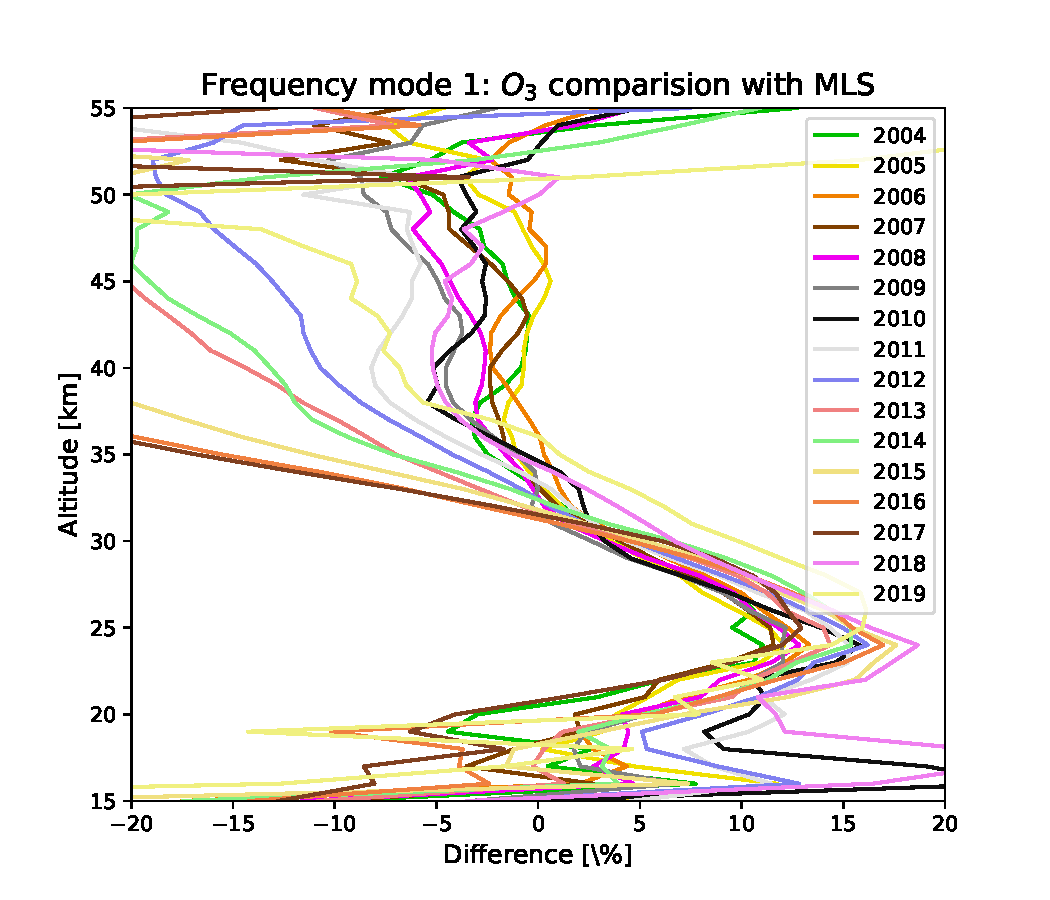
\includegraphics[width=\textwidth]{ALL-Strat-v3_0_0_fm1_O3_perdiff_mls}
        \caption{average difference to MLS}
        \label{fig:fm01:O3:profiles:MLS}
    \end{subfigure}

    \begin{subfigure}[b]{0.49\textwidth}
        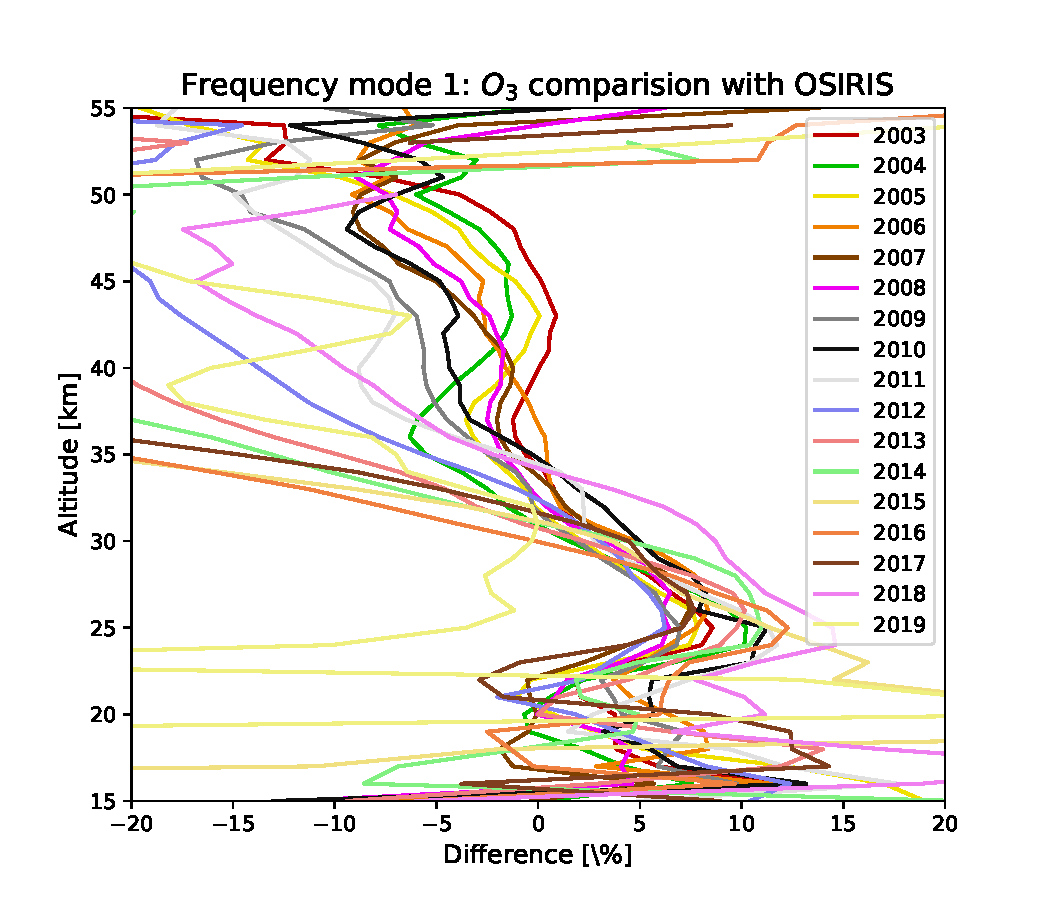
\includegraphics[width=\textwidth]{ALL-Strat-v3_0_0_fm1_O3_perdiff_osiris}
        \caption{average difference to OSIRIS}
        \label{fig:fm01:O3:profiles:OSIRIS}
    \end{subfigure}
    \,
    \begin{subfigure}[b]{0.49\textwidth}
        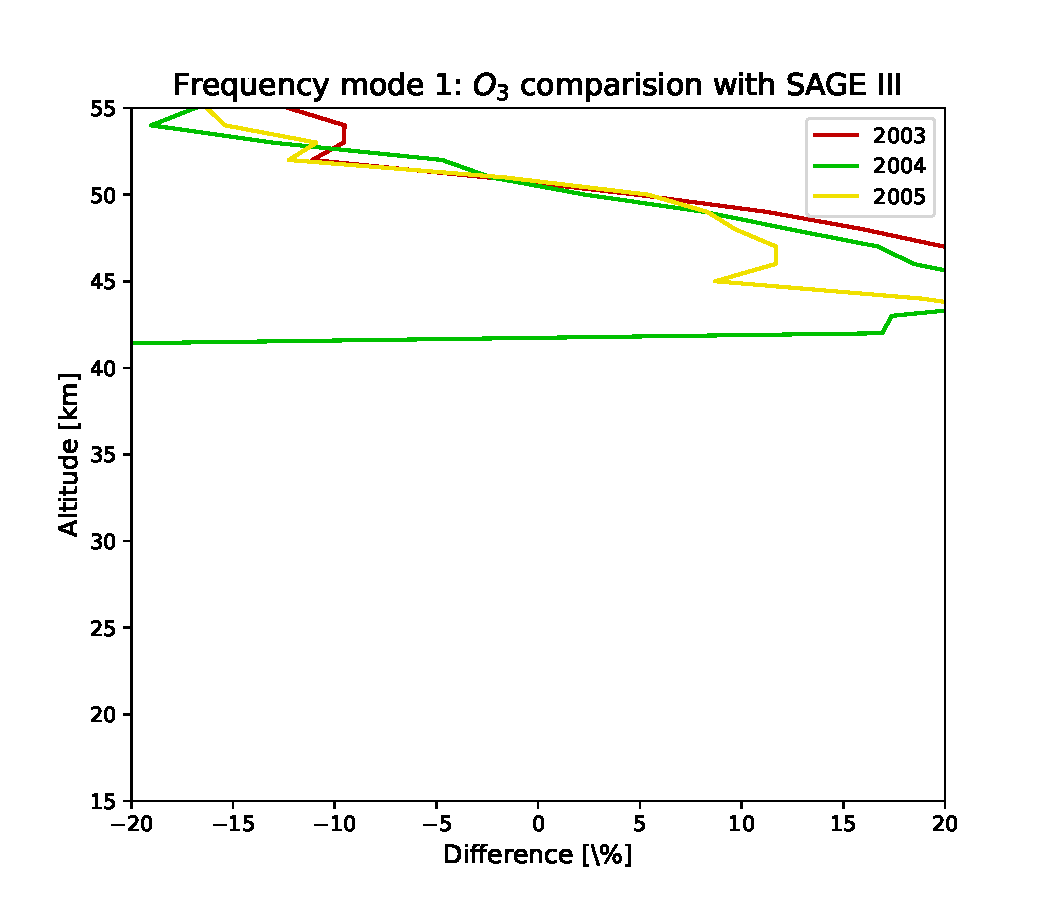
\includegraphics[width=\textwidth]{ALL-Strat-v3_0_0_fm1_O3_perdiff_sage}
        \caption{average difference to SAGEIII}
        \label{fig:fm01:O3:profiles:SAGEIII}
    \end{subfigure}
    \caption{Average difference in percent between retrievals of \chem{O_3}
    from \smr~v3 and collocated measurements from various instruments at
    different altitudes for frequency mode~01.}
    \label{fig:fm01:O3:profiles}
\end{figure}

\begin{figure}[tbhp]
    \centering
    \begin{subfigure}[b]{0.49\textwidth}
        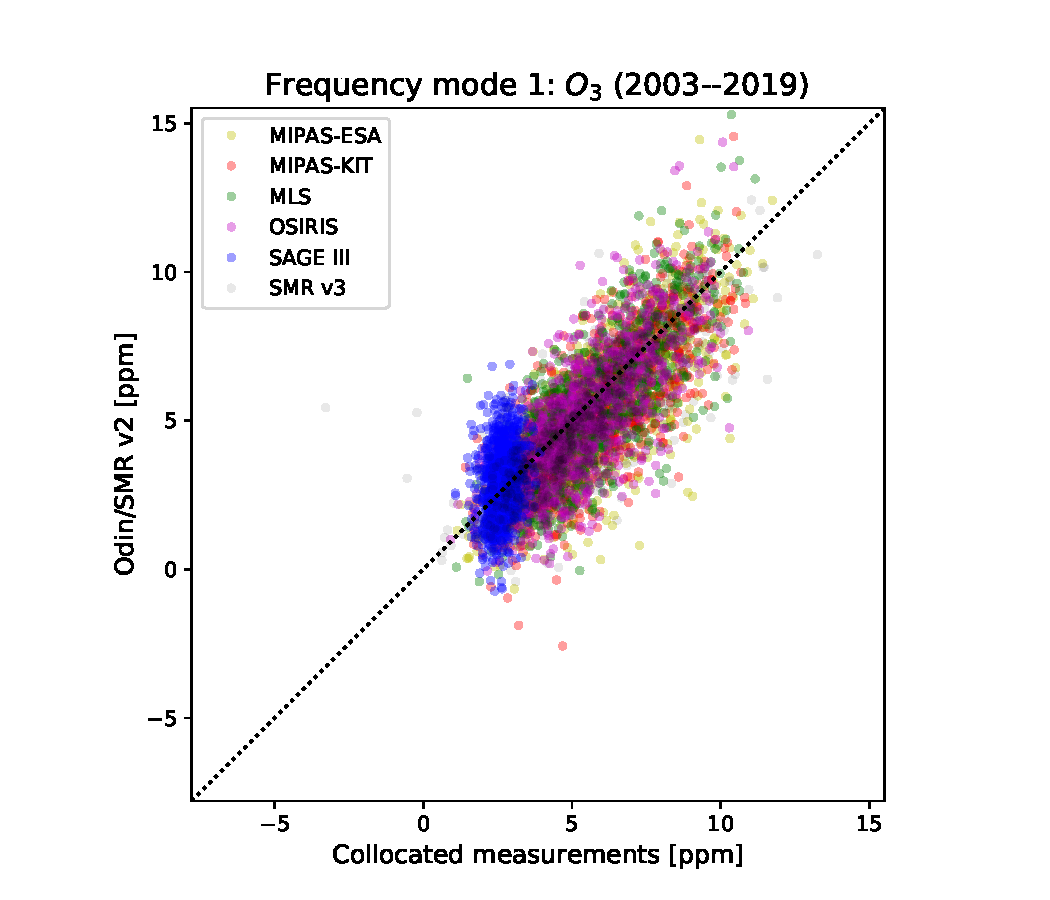
\includegraphics[width=\textwidth]{ALL-Strat-v3_0_0_fm1_O3_scatter_v2}
        \caption{correlation of collcated instruments with \smr~v2.X}
        \label{fig:fm01:O3:scatter:v2}
    \end{subfigure}
    \,
    \begin{subfigure}[b]{0.49\textwidth}
        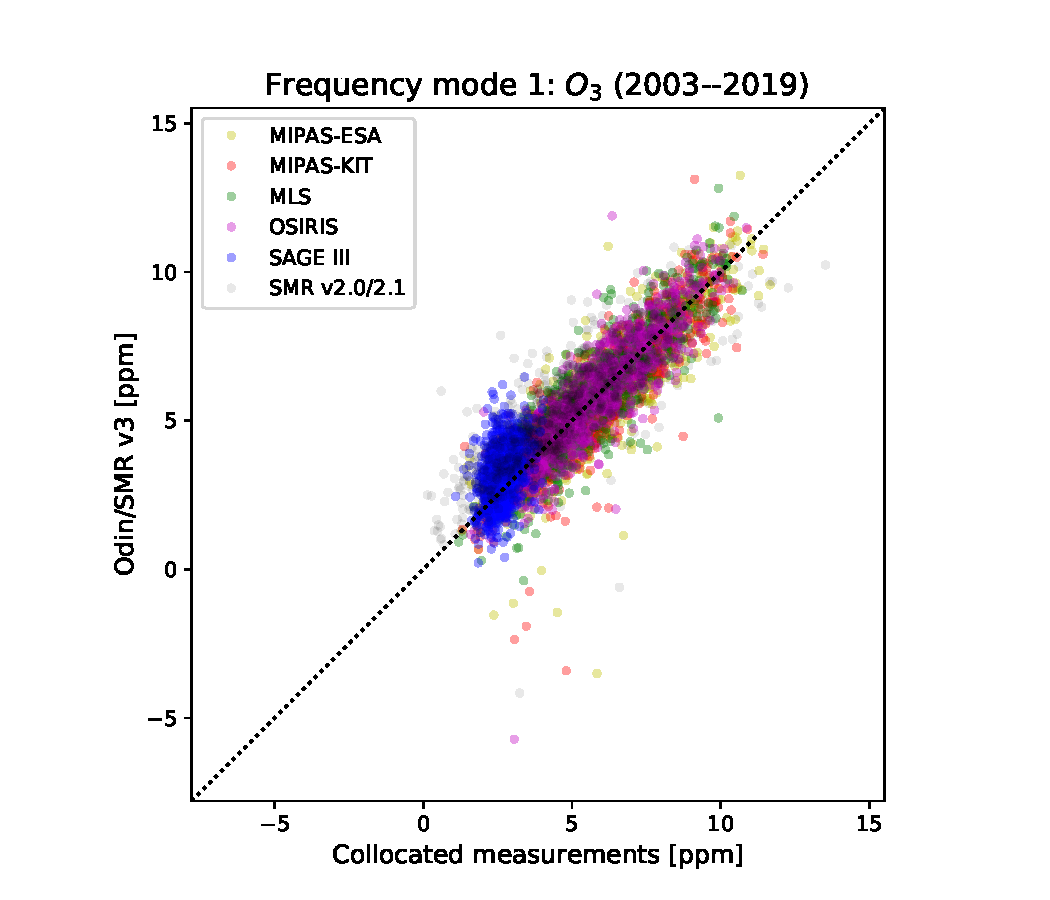
\includegraphics[width=\textwidth]{ALL-Strat-v3_0_0_fm1_O3_scatter_v3}
        \caption{correlation of collcated instruments with \smr~v3}
        \label{fig:fm01:O3:scatter:v3}
    \end{subfigure}
    \caption{Correlation between retrievals of \chem{O_3} using \smr\
    versions~2.X and~3 and collocated measurements from various instruments
    for frequency mode~01.} The period is restricted to 2003-2008 in order to avoid the errors caused by the LO from 2009 -2018.
    \label{fig:fm01:O3:scatter}
\end{figure}

\begin{figure}[tbhp]
    \centering
    \begin{subfigure}[b]{0.49\textwidth}
        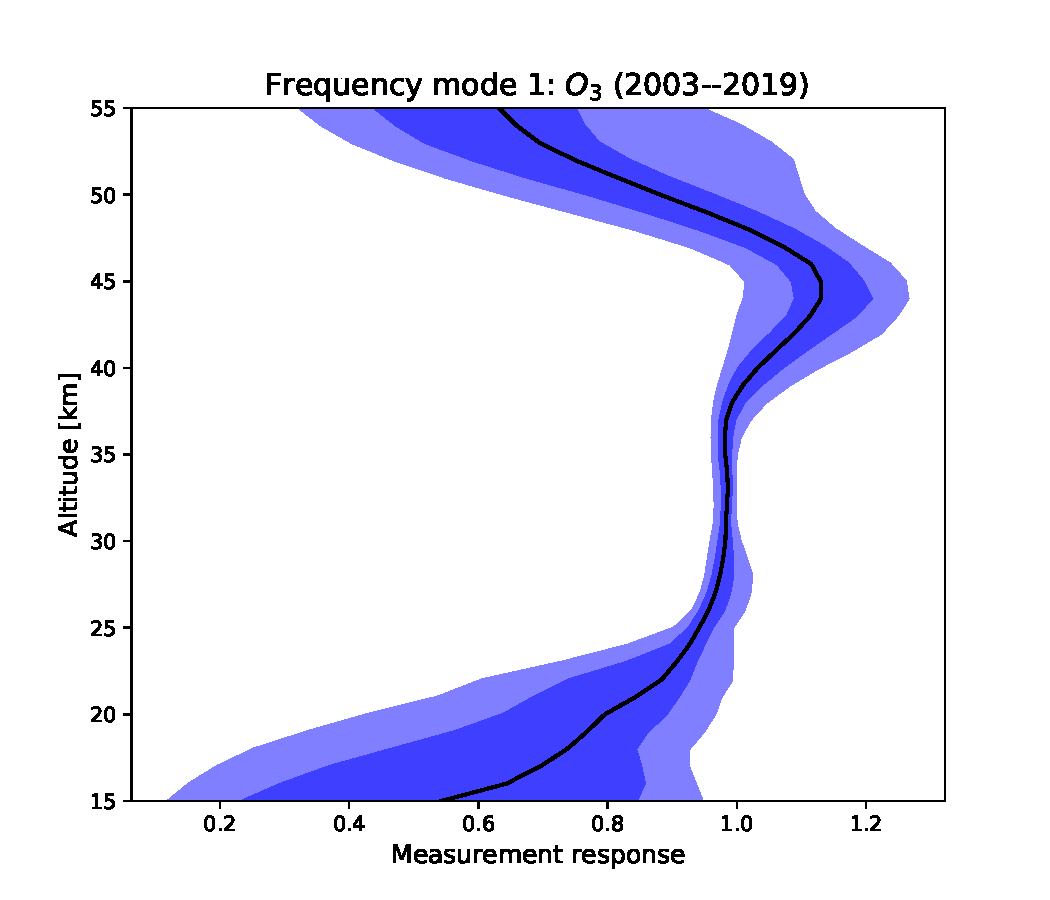
\includegraphics[width=\textwidth]{ALL-Strat-v3_0_0_fm1_O3_mr}
        \caption{median measurement response with $1\sigma$ and $2\sigma$
        percentiles}
        \label{fig:fm01:O3:mr}
    \end{subfigure}
    \,
    \begin{subfigure}[b]{0.49\textwidth}
        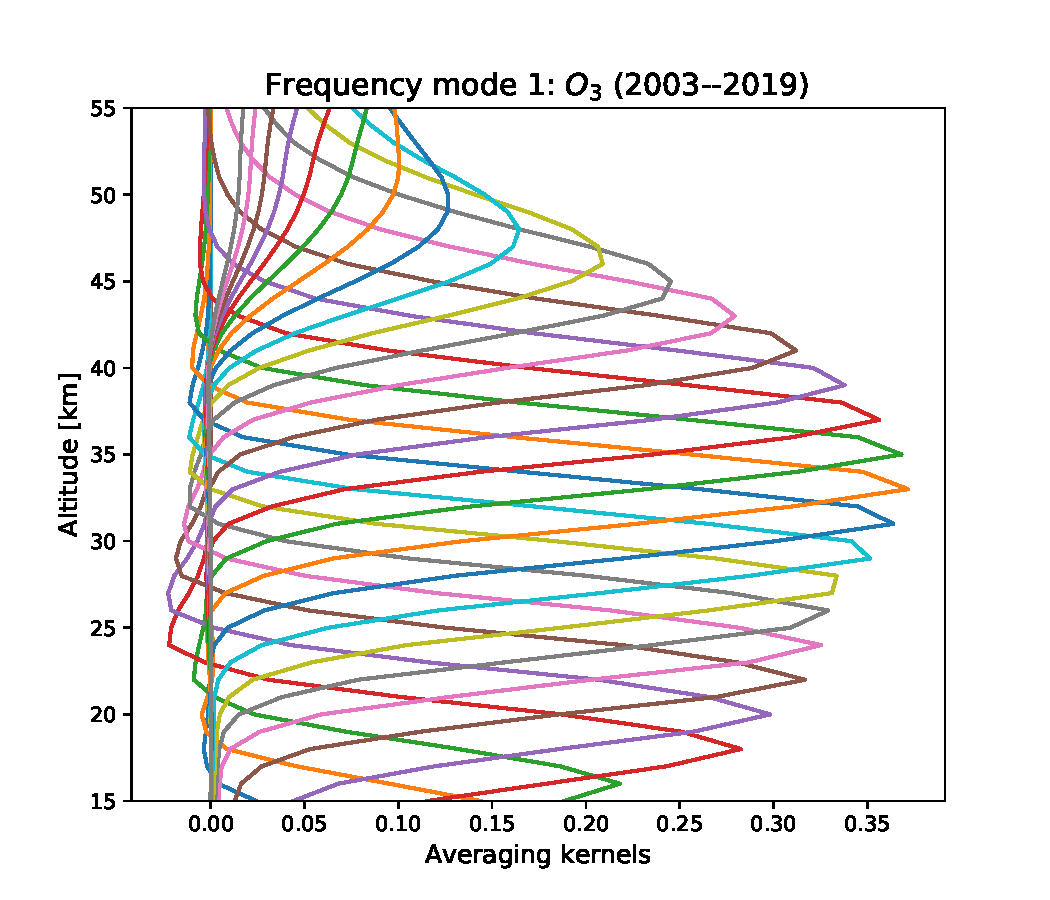
\includegraphics[width=\textwidth]{ALL-Strat-v3_0_0_fm1_O3_avk}
        \caption{median averaging kernels\newline~}
        \label{fig:fm01:O3:avk}
    \end{subfigure}
    \caption{Measurement response and averaging kernels for \chem{O_3}
    retrievals for \smr~v3 at different altitudes for frequency mode~01.}
    \label{fig:fm01:O3:mr_avk}
\end{figure}


%%%%%%%
% N2O %
%%%%%%%
\newpage
\subsubsection{\chem{N_2O}}
\label{sec:fm01:comparison:N2O}
The retrievals for \chem{N_2O} have been compared with data from the MIPAS and
MLS instruments. Annual average differences to these instruments are shown in
Figure~\ref{fig:fm01:N2O:profiles}. In Figure~\ref{fig:fm01:N2O:scatter}
individual retrievals for the instruments for the entire period are plotted
against the retrievals from the new and old versions of the \smr\ processing
chain. Only a minor improvement is seen with the updated version of the
processing. Figure~\ref{fig:fm01:N2O:mr_avk} suggests that the product is
useful over the range 15--50~km with a vertical resolution of around 5~km.


\begin{figure}[tbhp]
    \centering
    \begin{subfigure}[b]{0.49\textwidth}
        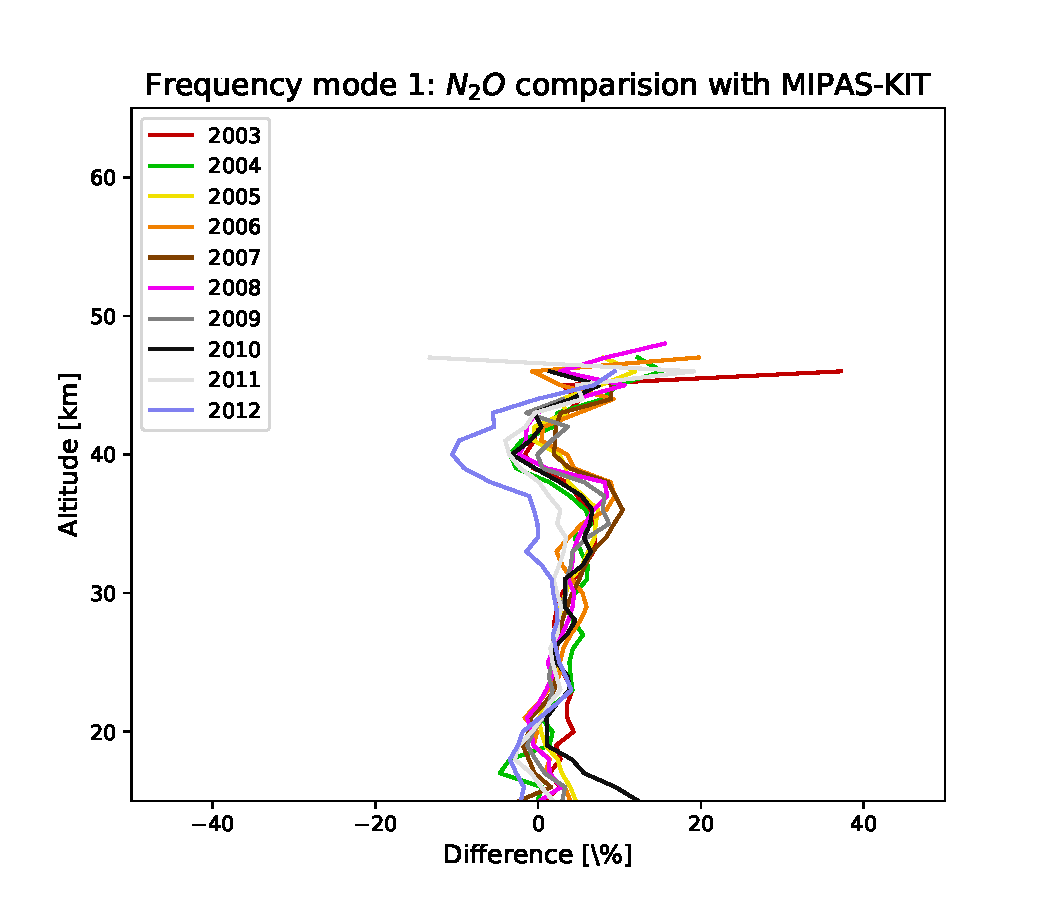
\includegraphics[width=\textwidth]{ALL-Strat-v3_0_0_fm1_N2O_perdiff_mipas}
        \caption{average difference to MIPAS}
        \label{fig:fm01:N2O:profiles:MIPAS}
    \end{subfigure}
    \,
    \begin{subfigure}[b]{0.49\textwidth}
        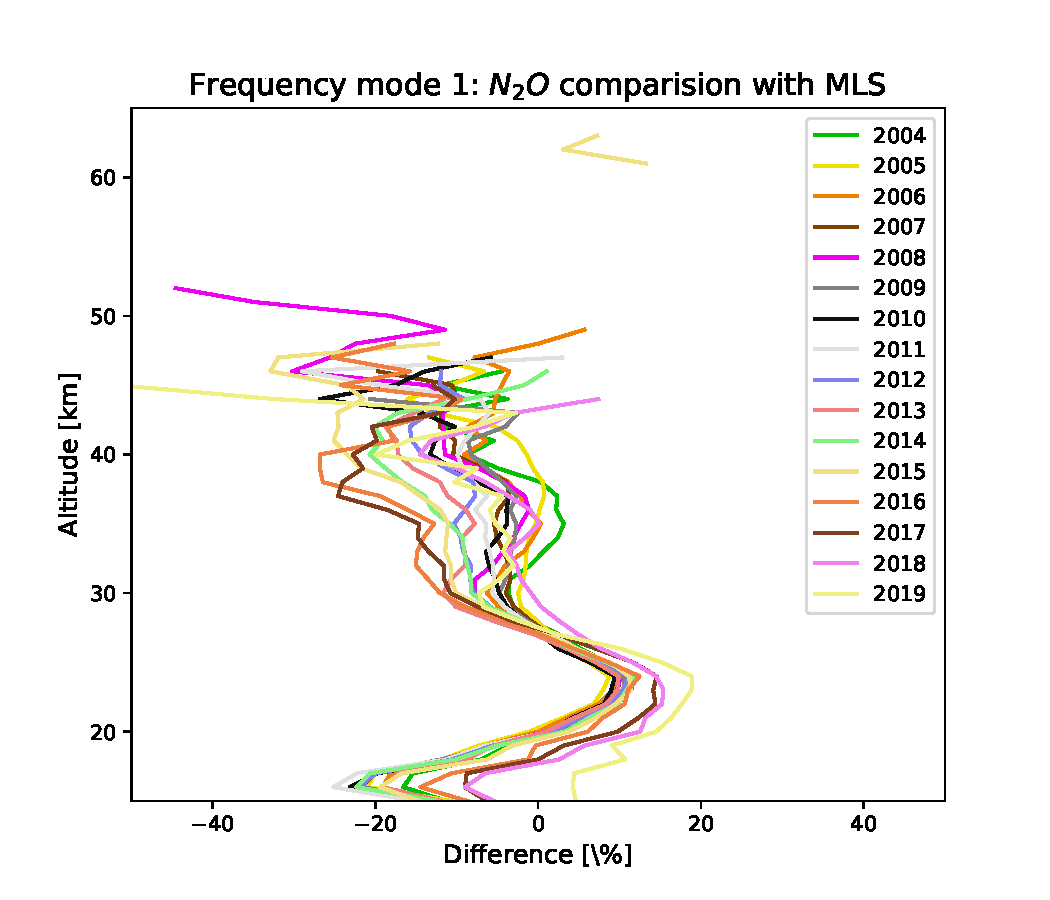
\includegraphics[width=\textwidth]{ALL-Strat-v3_0_0_fm1_N2O_perdiff_mls}
        \caption{average difference to MLS}
        \label{fig:fm01:N2O:profiles:MLS}
    \end{subfigure}
    \caption{Average difference in percent between retrievals of \chem{N_2O}
    from \smr~v3 and collocated measurements from various instruments at
    different altitudes for frequency mode~01. (Retrievals yielding
    concentrations $\leq 0.03\,\mathrm{ppm}$ have been filtered out.)}
    \label{fig:fm01:N2O:profiles}
\end{figure}

\begin{figure}[tbhp]
    \centering
    \begin{subfigure}[b]{0.49\textwidth}
        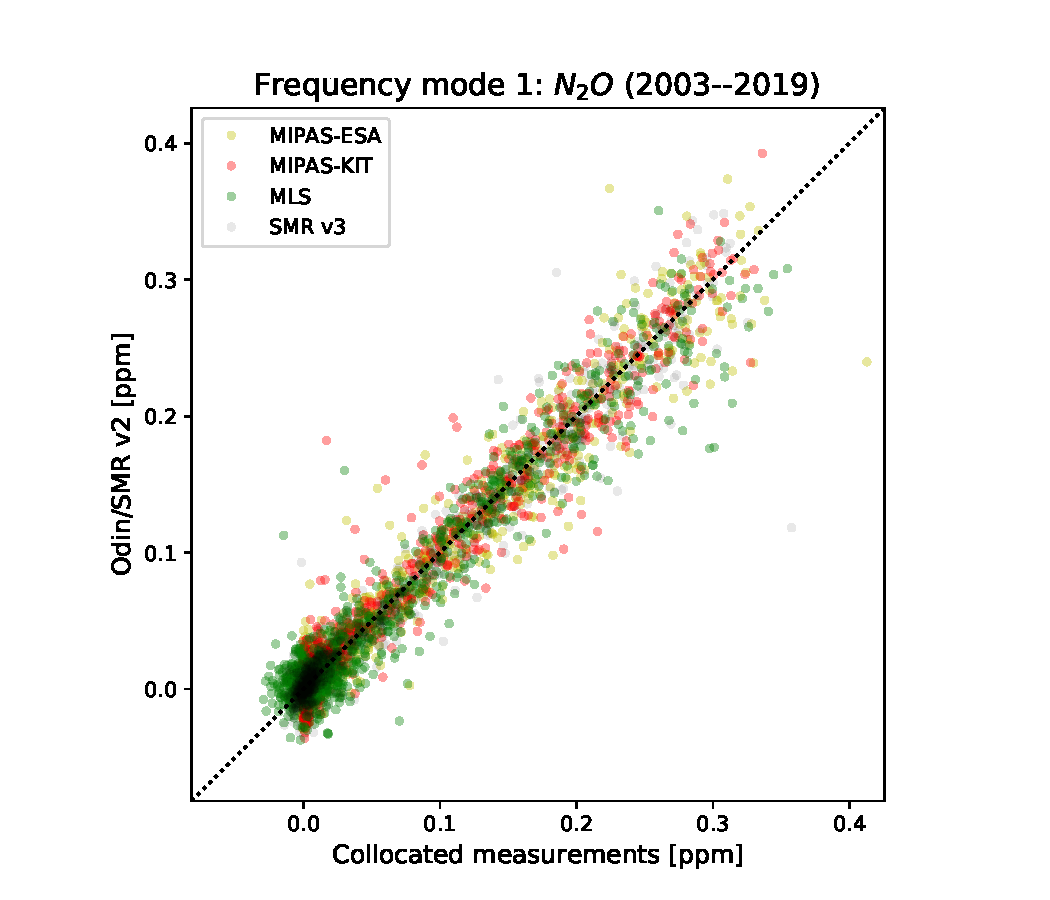
\includegraphics[width=\textwidth]{ALL-Strat-v3_0_0_fm1_N2O_scatter_v2}
        \caption{correlation of collcated instruments with \smr~v2.X}
        \label{fig:fm01:N2O:scatter:v2}
    \end{subfigure}
    \,
    \begin{subfigure}[b]{0.49\textwidth}
        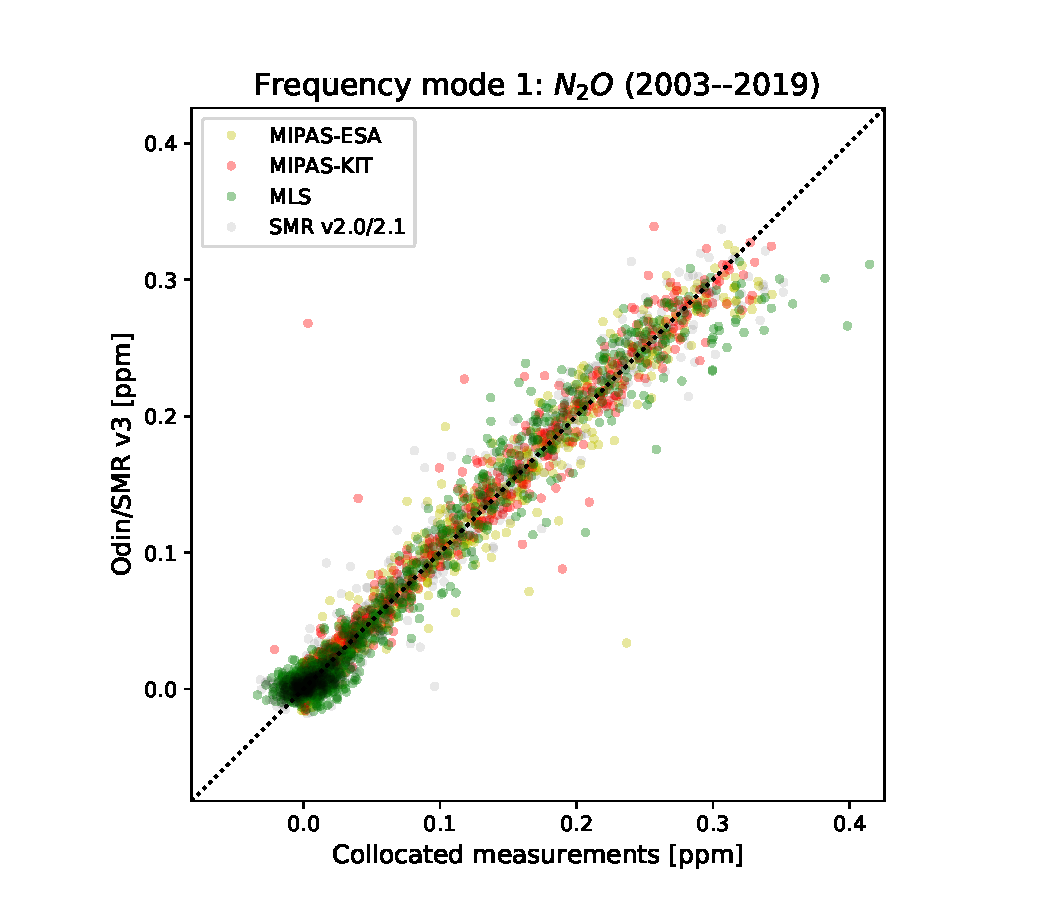
\includegraphics[width=\textwidth]{ALL-Strat-v3_0_0_fm1_N2O_scatter_v3}
        \caption{correlation of collcated instruments with \smr~v3}
        \label{fig:fm01:N2O:scatter:v3}
    \end{subfigure}
    \caption{Correlation between retrievals of \chem{N_2O} using \smr\
    versions~2.X and~3 and collocated measurements from various instruments
    for frequency mode~01.}
    \label{fig:fm01:N2O:scatter}
\end{figure}

\begin{figure}[tbhp]
    \centering
    \begin{subfigure}[b]{0.49\textwidth}
        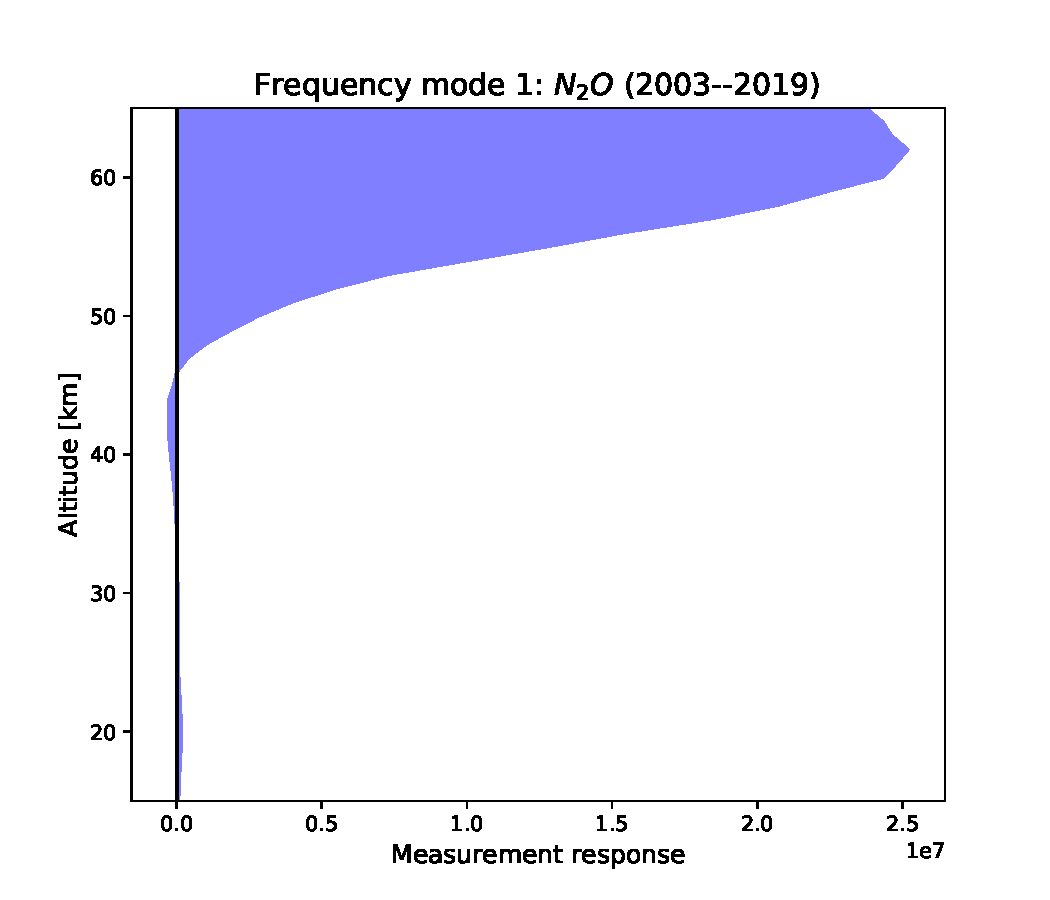
\includegraphics[width=\textwidth]{ALL-Strat-v3_0_0_fm1_N2O_mr}
        \caption{median measurement response with $1\sigma$ and $2\sigma$
        percentiles}
        \label{fig:fm01:N2O:mr}
    \end{subfigure}
    \,
    \begin{subfigure}[b]{0.49\textwidth}
        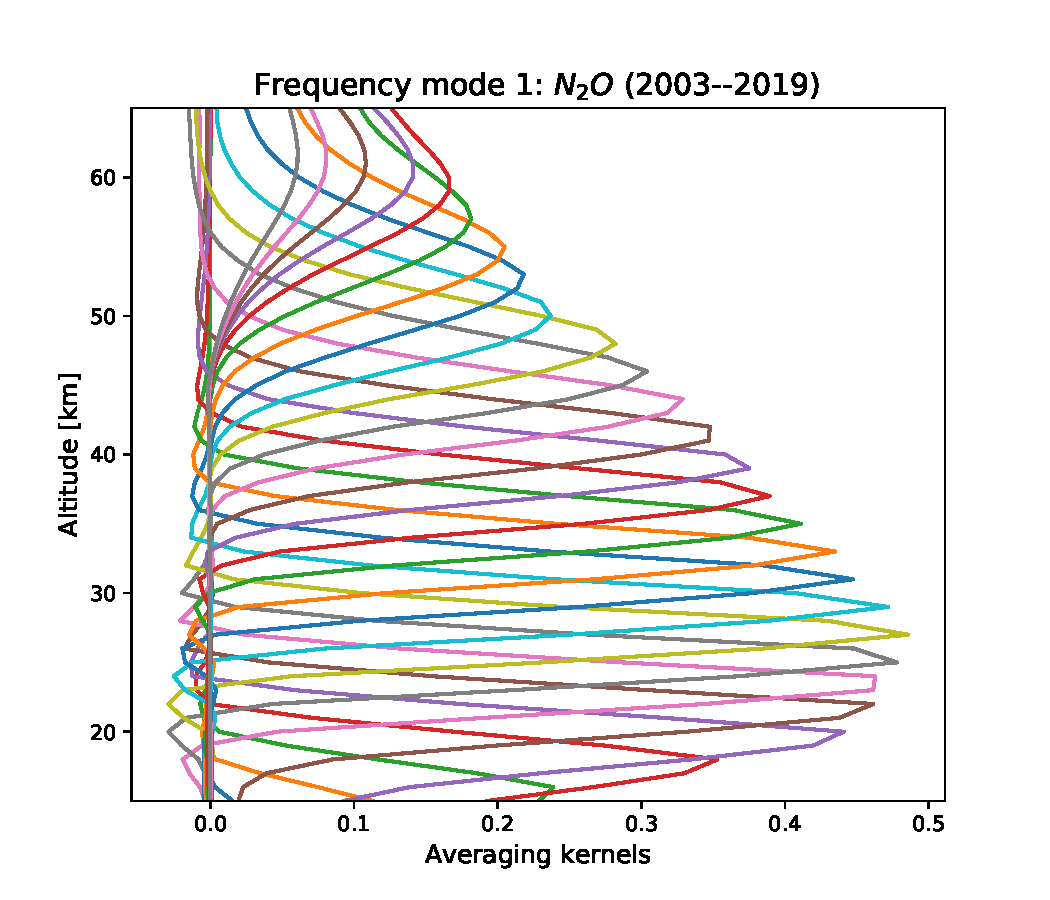
\includegraphics[width=\textwidth]{ALL-Strat-v3_0_0_fm1_N2O_avk}
        \caption{median averaging kernels\newline~}
        \label{fig:fm01:N2O:avk}
    \end{subfigure}
    \caption{Measurement response and averaging kernels for \chem{N_2O}
    retrievals for \smr~v3 at different altitudes for frequency mode~01.}
    \label{fig:fm01:N2O:mr_avk}
\end{figure}


%%%%%%%
% ClO %
%%%%%%%
\newpage
\subsubsection{\chem{ClO}}
\label{sec:fm01:comparison:ClO}
The retrievals for \chem{ClO} have been compared with data from the MLS
instrument. Annual average differences to MLS are shown in
Figure~\ref{fig:fm01:ClO:profiles}. In Figure~\ref{fig:fm01:ClO:scatter}
individual retrievals from MLS for the entire period are plotted against the
retrievals from the new and old versions of the \smr\ processing chain. No
sizeable improvement is seen for the new version of the \smr\ processing chain
compared to MLS, and the correlation and coherrency between the two remains
poor, however, Figure~\ref{fig:fm01:ClO:scatter} suggests that this is due to
noisy nature of the MLS retrievals, which show a very large spread -- sometimes
even large negative concentrations -- for the retrievals where both \smr\
versions yield low \chem{ClO} concentrations. A further  explanation is
that, since \chem{ClO} concentrations have a diurnal cycle, collocation in time
is very important for comparisons, and due to the orbits of the two
instruments, this is only really satisfied near the poles. In this comparison
we have not attempted to separate periods of chlorine activation from period
with a normal vertical distribution. From previous experience we know that the
dirunal effect can be very large in such comparisons.
Figure~\ref{fig:fm01:ClO:mr_avk} suggests that the product is useful in the
range 18--55~km with a vertical resolution of around 5~km.


\begin{figure}[tbhp]
    \centering
    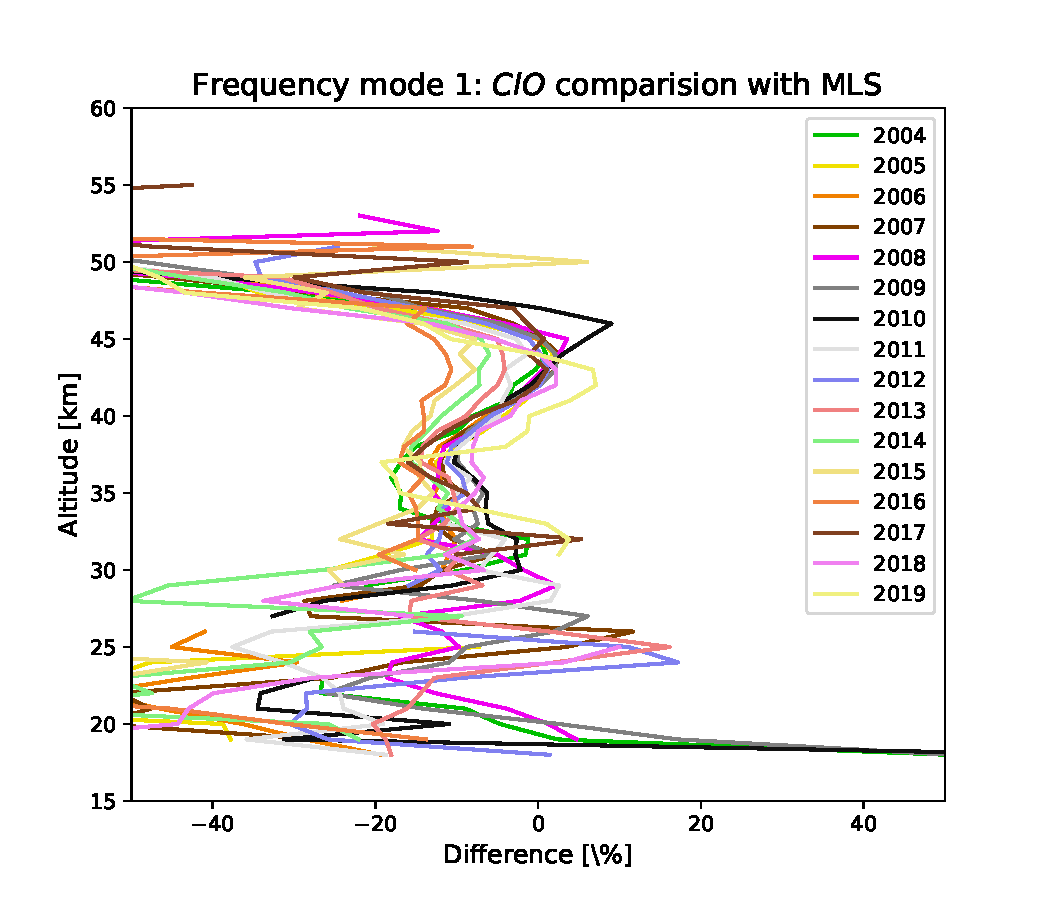
\includegraphics[width=0.618\textwidth]{ALL-Strat-v3_0_0_fm1_ClO_perdiff_mls}
    \caption{Average difference in percent between retrievals of \chem{ClO}
    from \smr~v3 and collocated measurements from MLS at
    different altitudes for frequency mode~01. (Retrievals yielding
    concentrations $\leq 0.3\,\mathrm{ppb}$ have been filtered out.)}
    \label{fig:fm01:ClO:profiles}
    \label{fig:fm01:ClO:profiles:MLS}
\end{figure}

\begin{figure}[tbhp]
    \centering
    \begin{subfigure}[b]{0.49\textwidth}
        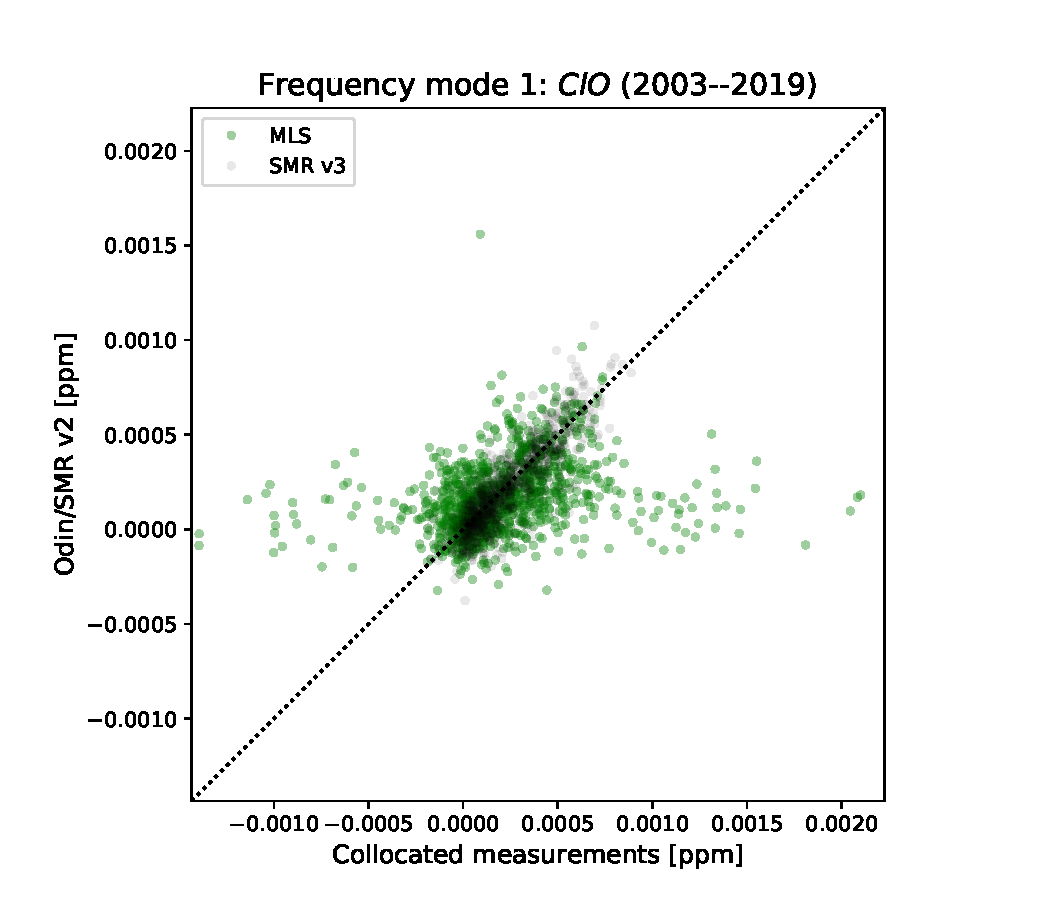
\includegraphics[width=\textwidth]{ALL-Strat-v3_0_0_fm1_ClO_scatter_v2}
        \caption{correlation of collcated MLS measurements with \smr~v2.X}
        \label{fig:fm01:ClO:scatter:v2}
    \end{subfigure}
    \,
    \begin{subfigure}[b]{0.49\textwidth}
        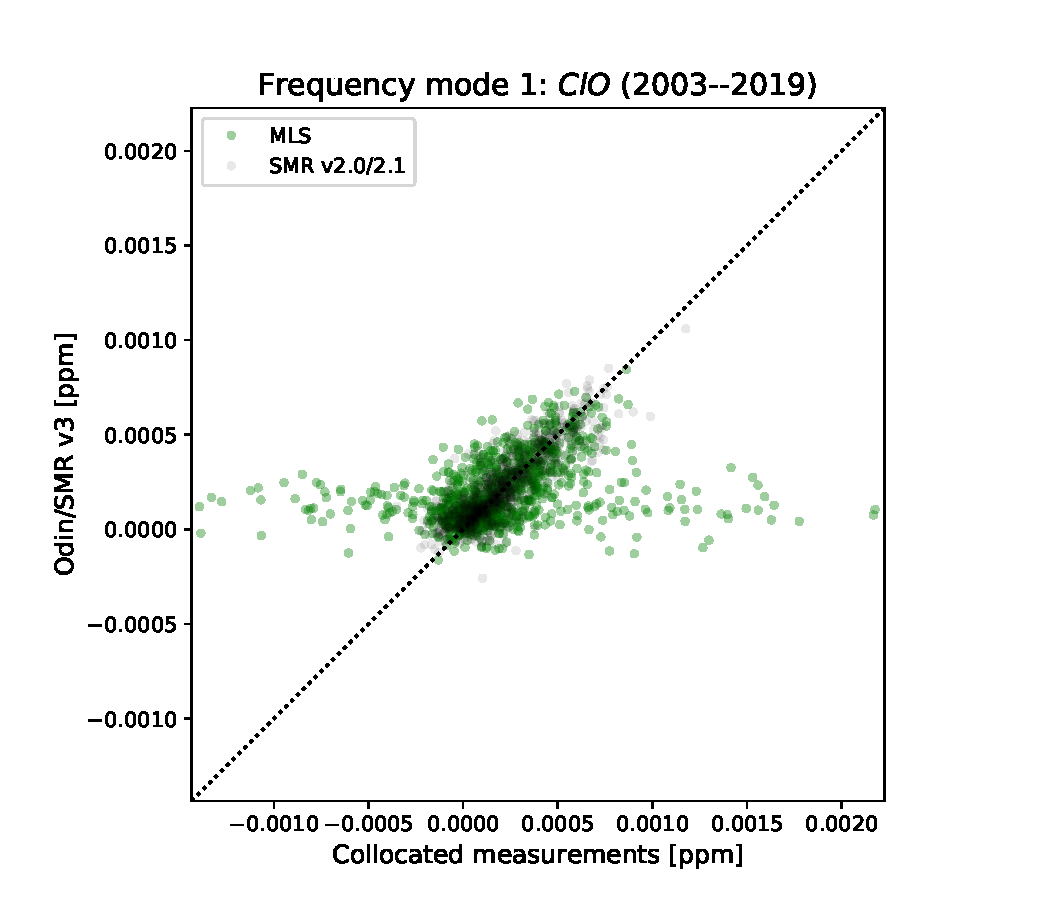
\includegraphics[width=\textwidth]{ALL-Strat-v3_0_0_fm1_ClO_scatter_v3}
        \caption{correlation of collcated MLS measurements with \smr~v3}
        \label{fig:fm01:ClO:scatter:v3}
    \end{subfigure}
    \caption{Correlation between retrievals of \chem{ClO} using \smr\
    versions~2.X and~3 and collocated measurements MLS for frequency mode~01.}
    \label{fig:fm01:ClO:scatter}
\end{figure}

\begin{figure}[tbhp]
    \centering
    \begin{subfigure}[b]{0.49\textwidth}
        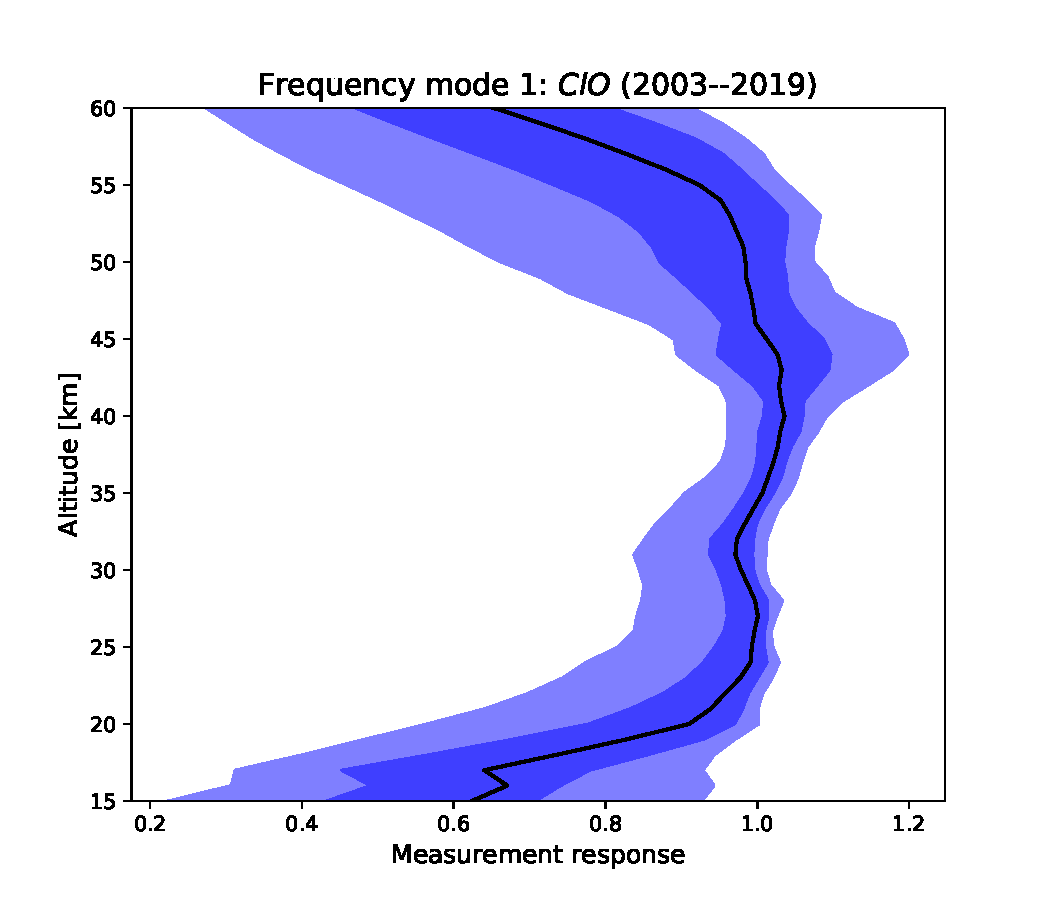
\includegraphics[width=\textwidth]{ALL-Strat-v3_0_0_fm1_ClO_mr}
        \caption{median measurement response.  $1\sigma$ and $2\sigma$
        percentiles are also shown}
        \label{fig:fm01:ClO:mr}
    \end{subfigure}
    \,
    \begin{subfigure}[b]{0.49\textwidth}
        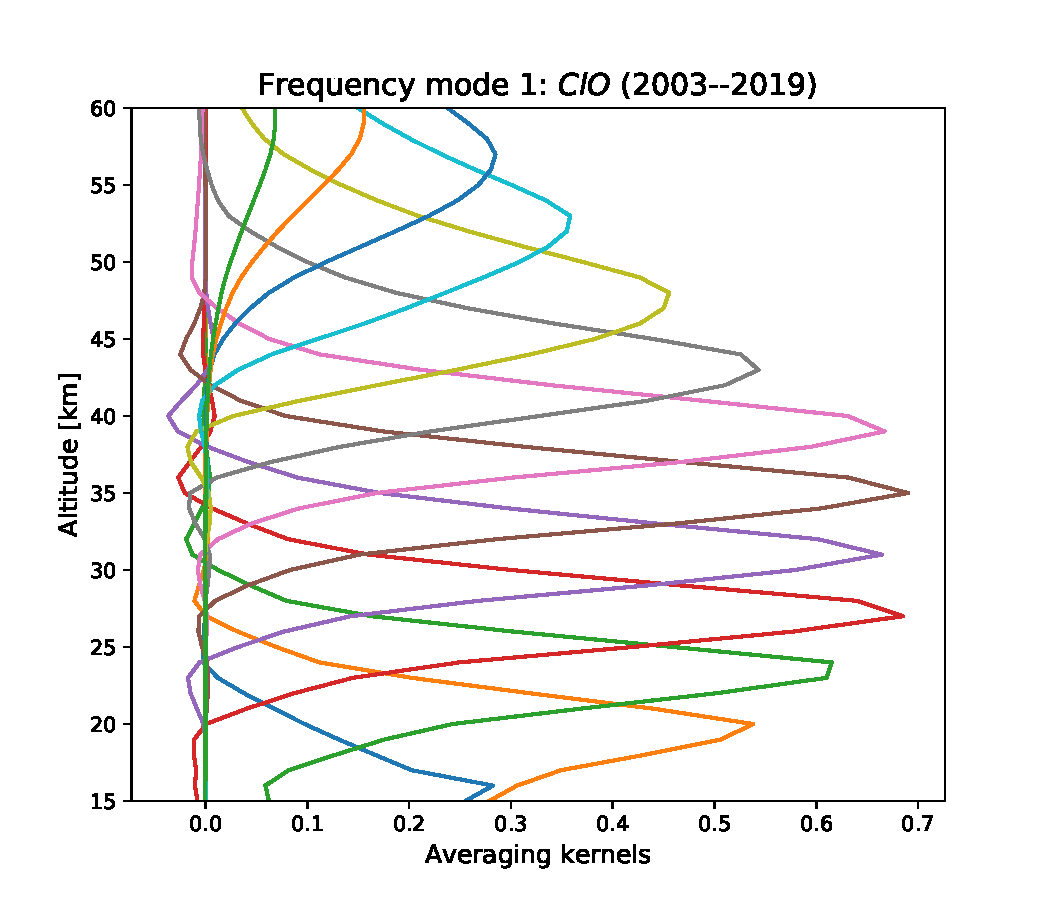
\includegraphics[width=\textwidth]{ALL-Strat-v3_0_0_fm1_ClO_avk}
        \caption{median averaging kernels\newline~}
        \label{fig:fm01:ClO:avk}
    \end{subfigure}
    \caption{Measurement response and averaging kernels for \chem{ClO}
    retrievals for \smr~v3 at different altitudes for frequency mode~01.}
    \label{fig:fm01:ClO:mr_avk}
\end{figure}

\newpage
\subsection{Discussion}
\label{sec:fm01:discussion}
The Pearson correlation between the \smr\ retrievals and the other instruments
was calculated for the overlap periods for both versions of the processing
chain.  The results are summarised in Table~\ref{tab:fm01:stats}, and show that
the new algorithm is an improvement compared to all the instruments (with the
exception of SAGE) for all species used in this investigation. The improvement
is considerable for the \chem{O_3}, but only slight for \chem{N_2O}
and~\chem{ClO}, with the latter still showing very poor correlation with the
collocated MLS data. Correlations and fits were also calculated for the
individual years in the period (see~Figure~\ref{fig:fm01:O3:corr}), but no
trends of note were seen until 2009, when a instrument problem occurred or
possibly increased which renders retrievals from frequency mode~01 unreliable
outside the arctic summer months.  The problem caused asymmetric broadening of
the lines resulting in bad fits and reduced species concentrations. It may be
possible to compensate for the effect in a later reprocessing and rescue the
data but this is not yet clear. The problem was fixed late in 2017 through
retuning of driving circuits by the instrument scientist.  Averaging of some
weeks of spectra show that the distortions of the lines has been removed.


\begin{table}[tbhp]
\centering
\caption{Pearson correlation and fit parameters of the old and new \smr\
retrievals for frequency mode~01, compared with collocated data from other
instruments for the period 2003--2019.
$\left|\left<\right.\right.$res.$\left.\left.\right>\right|$ is the mean
residual.}
\label{tab:fm01:stats}
\begin{tabular}{lllrrrr}
    \toprule
    \textbf{Species} & \textbf{Instrument} & \textbf{SMR} & \textbf{corr.} & \textbf{slope} & \textbf{intercept} & \textbf{$\left|\left<\right.\right.$res.$\left.\left.\right>\right|$} \\
    \midrule
    \chem{O3}   & MIPAS (KIT)   & v3    & 0.900 & 0.979 & 0.044\,ppm    &  1.056\,ppm \\
                &               & v2.x  & 0.789 & 0.908 & 0.007\,ppm    &  1.497\,ppm \\
    \cline{2-7}
                & MIPAS (ESA)   & v3    & 0.887 & 0.959 & 0.108\,ppm    &  1.128\,ppm \\
                &               & v2.x  & 0.778 & 0.885 & 0.098\,ppm    &  1.548\,ppm \\
    \cline{2-7}
                & MLS           & v3    & 0.898 & 0.999 & 0.129\,ppm    &  1.030\,ppm \\
                &               & v2.x  & 0.778 & 0.923 & 0.095\,ppm    &  1.436\,ppm \\
    \cline{2-7}
                & OSIRIS        & v3    & 0.918 & 1.005 &  0.053\,ppm   &  0.890\,ppm \\
                &               & v2.x  & 0.783 & 0.951 & -0.101\,ppm   &  1.426\,ppm \\
    \cline{2-7}
                & SAGE III      & v3    & 0.439 & 1.023 & 0.371\,ppm    &  0.943\,ppm \\
                &               & v2.x  & 0.275 & 0.840 & 0.654\,ppm    &  1.193\,ppm \\
    \midrule
    \chem{N_2O} & MIPAS (KIT)   & v3    & 0.983 & 0.985 & 2.844\,ppb    & 16.750\,ppb \\
                &               & v2.x  & 0.975 & 0.979 & 2.786\,ppb    & 20.055\,ppb \\
    \cline{2-7}
                & MIPAS (ESA)   & v3    & 0.017 & 0.000 & 67.659\,ppb   & 19.677\,ppm \\
                &               & v2.x  & 0.086 & 0.007 & 67.000\,ppb   &  1.148\,ppm \\
    \cline{2-7}
                & MLS           & v3    & 0.976 & 0.960 & 2.062\,ppb    & 19.809\,ppb \\
                &               & v2.x  & 0.968 & 0.940 & 2.632\,ppb    & 22.881\,ppb \\
    \midrule
    \chem{ClO}  & MLS           & v3    & 0.259 & 0.098 & 0.177\,ppb    &  0.436\,ppb \\
                &               & v2.x  & 0.238 & 0.109 & 0.160\,ppb    &  0.441\,ppb \\
    \bottomrule
\end{tabular}
\end{table}

\begin{figure}[ht]
    \centering
    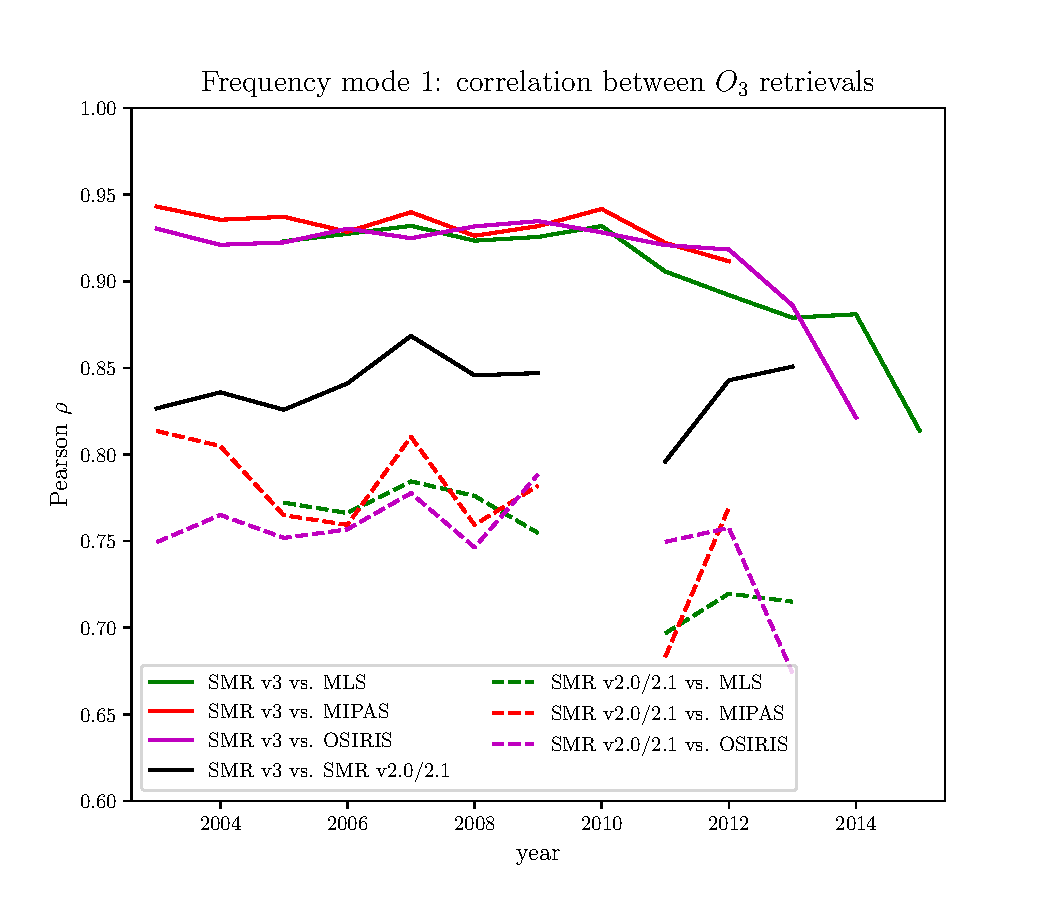
\includegraphics[width=0.618\textwidth]{../DDS/figures/DDS_fm1_O3_corr}
    \caption{Pearson correlation ($\rho$) of \smr~v3~(---) and~v2.X~(--~--)
    retrievals of \chem{O_3} with collocated measurements. Note the decline in
    $\rho$ after 2009.}
    \label{fig:fm01:O3:corr}
\end{figure}

\subsection{Conclusions}
\label{sec:fm01:conclusions}
Based on the discussion above, retrievals based on frequency mode~01 can be
used with confidence for the species~\chem{O_3} and~\chem{N_2O} for the
period 2003--2008. Retrievals of \chem{ClO} based on this frequency mode
should be used with some caution taking account of the local time of the
observations.

For the period 2009--2017  all retrievals from frequency mode~01 should be used
with  caution, if at all, due to the problem discussed
in~Sec.~\ref{sec:fm01:discussion}. The only exceptions are retrievals from the
middle of the arctic summer, which are not affected by this problem as a result
of the satelite being colder during this period~\cite{postlaunch:2006}. The
problem was fixed in late 2017, wherefore data from 2018 and onwards should
have the same quality as that of 2003--2008. This is confirmed by the comparisons.